%!TEX root = slides.tex

\section[Session 2]{Session 2: Empirical methods with which to detect
environmental and phenotypic associations: single and multiple locus
methodologies}

\begin{frame}
\frametitle{Fixed vs random effects}
\begin{block}{Fixed effects}
\begin{itemize}
\item{\textbf{Treatment} effects}
\item{Case vs. control, and \textbf{only} these two groups}
\item{Variable for which all levels are included (e.g., gender, race)}
\item{Explicitly compare between levels without generalizing (e.g., San
Francisco vs. Berkeley)}
\item{Usually qualitative variables}
\end{itemize}
\end{block}
\tiny
\citet{StroupFreund200203}
\end{frame}


\begin{frame}
\frametitle{Fixed vs random effects}
\begin{block}{Random effects}
\begin{itemize}
\item{Drawn from a distribution of possible effects}
\item{San Francisco and Berkeley are just two of many western US, 
or liberal, or hippie, or measels-infected cities}
\item{Use of a random effect allows for more generalizable conclusions 
from the data}
\item{rather than comparing among levels for an effect, random 
effects measure how much variance in the dependent variable is 
accounted for across levels of the random factor}
\item{Blocking, control, repeated-measures factors are random}
\end{itemize}
\end{block}
\tiny
\citet{StroupFreund200203}
\end{frame}



\begin{frame}
\frametitle{Detecting and dealing with population structure}
\begin{block}{Why is this important?}
\begin{itemize}
	\item{Can lead to spurious associations if not accounted for}
	\item{Population structure can look like LD}
	\item{Substantial and varying LD present in genome-scale datasets}
	\item{Which markers to use to access structure? - all of them}
	\item{Leave-one-out testing?}
\end{itemize}
\end{block}
\tiny
\citet{Price:2006cd}
\end{frame}

\begin{frame}
\frametitle{Multiple testing approaches}
\begin{block}{Methods}
\begin{itemize}
	\item Bonferroni
	\item Bootstrapping
	\item FDR
\end{itemize}
\end{block}
\end{frame}

\begin{frame}
\frametitle{Detecting and dealing with population structure}
\begin{block}{}
\centering
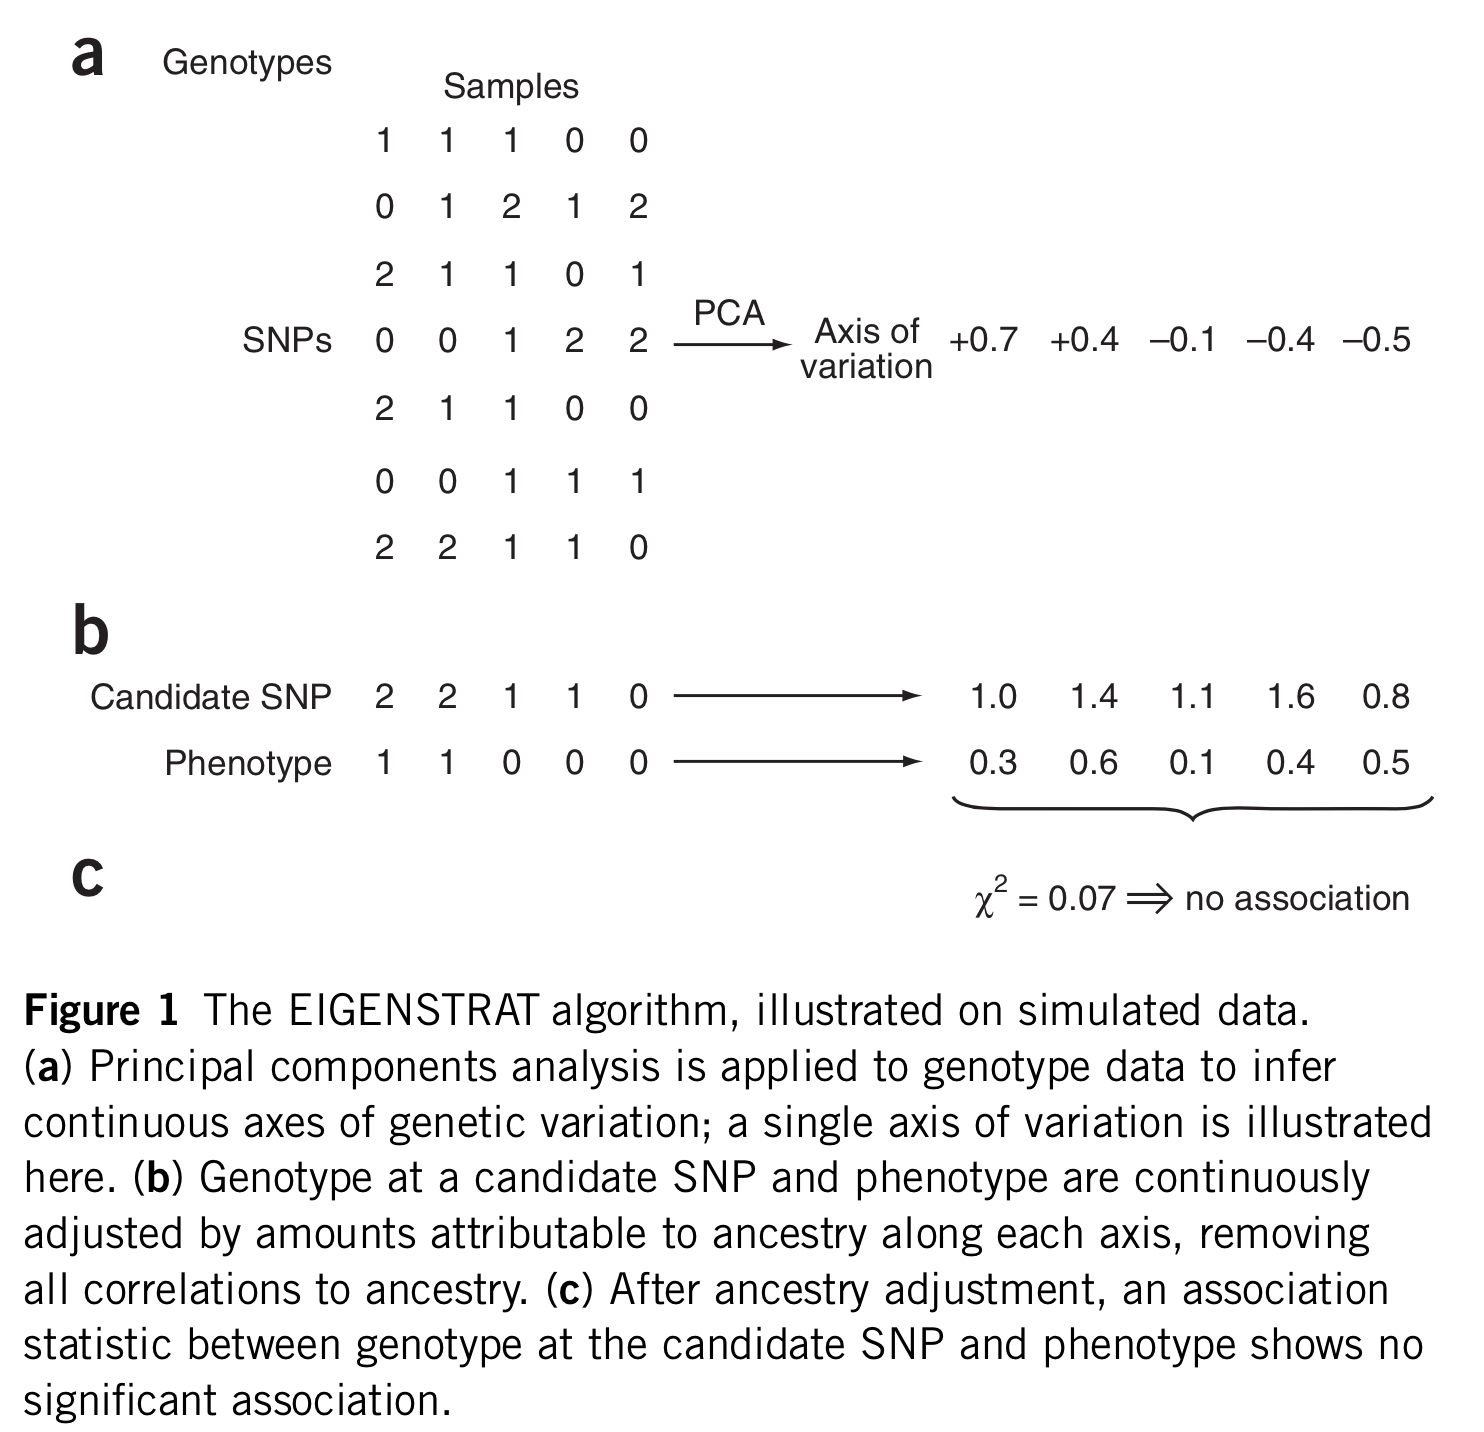
\includegraphics[height=0.8\textheight]{price.png}\\
\tiny
\citet[Figure 1]{Price:2006cd}
\end{block}
\end{frame}

\begin{frame}
\frametitle{Testing SNPs against phenotypes}
\begin{block}{}
\begin{center}
\Large{$y=X \bm{\beta} + S \bm{\alpha} + Q \bm{v} + Z \bm{u} + \bm{e}$}
\end{center}
\begin{itemize}
\item{$X \beta$: fixed effects w/o SNP + population structure}
\item{$\beta$: fixed effects other than SNP or pop. structure}
\item{$\alpha$: vector of SNP effects}
\item{$v$: vector of population effects}
\item{$u$: vector of polygene background effects}
\item{$Q$: matrix from STRUCTURE relating y to v}
\item{$X, S, Z$: incidence matrices (0/1) relating y to $\beta$, $\alpha$, $u$,
respectively}
\end{itemize}
\end{block}
\tiny
\citet{Yu:2006ij}
\end{frame}

\begin{frame}
\frametitle{Testing SNPs against phenotypes}
\begin{block}{}
\begin{center}
\Large{$y=X \bm{\beta} + S \bm{\alpha} + Q \bm{v} + Z \bm{u} + \bm{e}$}
\end{center}
\begin{itemize}
\item{$Var(u) = 2KV_g, Var(e) = RV_R$}
\item{$K$: $n \times n$ matrix of genetic covariance between pairs of
individuals (kinship)}
\item{$R$: $n \times n$ matrix off-diag elems are 0, diag is
$1/N_{{obs}_{pheno}}$}
\item{$V_g$: genetic variance (additive)}
\item{$V_R$: residual variance (non-additive + env)}
\end{itemize}
\end{block}
\tiny
\citet{Yu:2006ij}
\end{frame}

\begin{frame}
\frametitle{Bayenv: identifying correlations with ecological
variables}
\begin{block}{Basic Bayesian}
\begin{equation}
P(H | D) = \frac{P(D|H)P(H)}{P(D)}	
\end{equation}
\begin{equation}
P(H|D) \propto P(D|H)P(H)
\end{equation}
\begin{equation}
\frac{P(H_1|D)}{P(H_0|D)}
\end{equation}
\end{block}
\end{frame}


\begin{frame}
\frametitle{Bayenv: identifying correlations with ecological
variables}
\begin{block}{Comparing allele frequencies and the environment}
\begin{itemize}
\item{Given different environments, local adaptation should drive changes in
allele frequencies among populations}
\item{However, allele frequency differences can be artifacts.}
\item{Bayenv (and Bayenv2):}
\begin{itemize}
\item{Accounts for complications due to demography and uneven sampling}
\item{Reports Bayes factors, and correlation statistics for SNPs}
\item{Provides standardized allele frequencies with demographic features
approximately removed, which can be used in other statistical frameworks
to test for environmental correlations}
\item{Bayenv2 can also account for sampling variance in pooled populations}
\end{itemize}
\end{itemize}
\end{block}
\tiny
\citet{Gunther:2013ik, COOP:2010ke}
\end{frame}


\begin{frame}
\frametitle{Bayenv: identifying correlations with ecological
variables}
\begin{block}{Output}
\begin{itemize}
\item{Standardized allele frequencies}
\item{Detect SNP outliers while accounting for population history ($X^TX$)}
\end{itemize}
\end{block}
\end{frame}

\begin{frame}
\frametitle{Bayenv: identifying correlations with ecological
variables}
\begin{block}{}
\centering
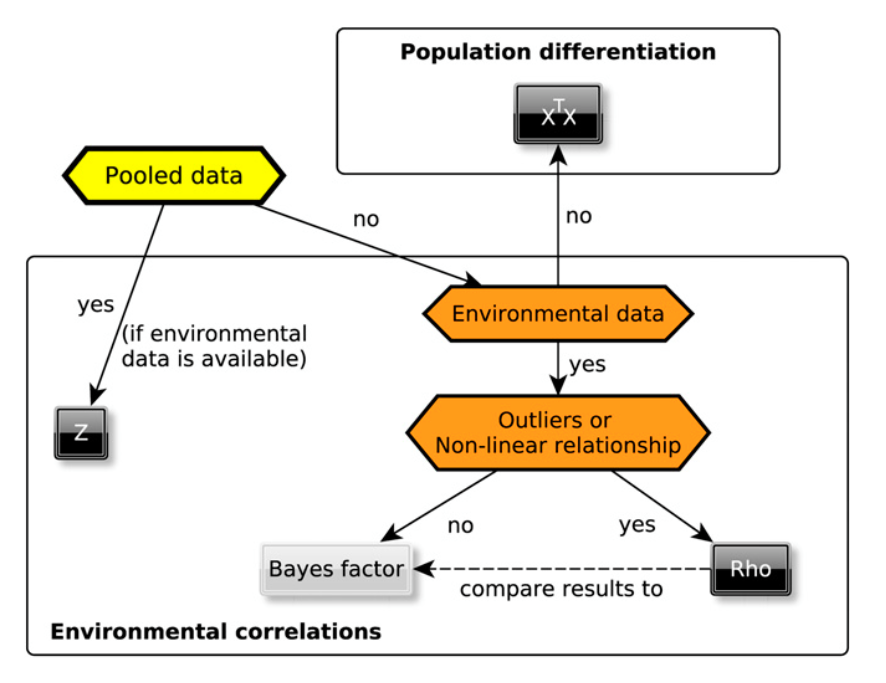
\includegraphics[width=.7\textwidth]{bayenv1}
\end{block}
\end{frame}

\begin{frame}
\frametitle{Bayenv: identifying correlations with ecological
variables}
\begin{block}{The method}
\begin{enumerate}
\item{Estimation of an empirical covariance matrix from allele count data from
L across K populations}
\item{Models joint distribution of allele frequencies across populations}
\begin{equation}
x_{kl} = g(\theta_{kl}) = \begin{cases}
	0 & \theta_{kl} < 0 \\
	\theta_{kl} & 0 \le \theta_{kl} < 1 \\
	1 & \theta_{kl} > 1
\end{cases}	
\end{equation}
\item{Point masses at 0 and 1 represent loss or gain, $\theta_l$ are MVN}
\begin{equation}
	P(\theta_l|\Omega, \epsilon_l) \sim
 N(\epsilon_l,\epsilon_l(1-\epsilon_l)\Omega)
\end{equation}
\end{enumerate}
\end{block}
\end{frame}


\begin{frame}
\frametitle{Bayenv: identifying correlations with ecological
variables}
\begin{block}{The method}
\begin{itemize}
\item{The joint posterior of $\Omega$ at a single locus is:}
\begin{equation}
P(\theta_1, \Omega, \epsilon_l | 
\bm{n}_1, \bm{m}_1) \propto \bm{n}_l,\bm{m}_l | x_l = g(\theta_l))
P(\theta_l | \Omega,\epsilon_l)P(\epsilon_l)P(\Omega)	
\end{equation}
\item{This is the null model of SNP frequencies across populations}
\item{Given this model, how are allele frequencies at SNPs correlated with 
the environmental variable(s), $Y$?}
\end{itemize}
\end{block}
\end{frame}


\begin{frame}
\frametitle{Bayenv: identifying correlations with ecological
variables}
\begin{block}{The method}
\begin{itemize}
\item{The joint posterior of $\Omega$ over all loci is:}
\begin{multline}
P(\Omega, \theta_1, \ldots , \theta_l, 
\epsilon_1, \ldots , \epsilon_L | 
\bm{n}_1, \bm{m}_1, \ldots , \bm{n}_L, \bm{m}_L) \\
\propto \left \{ \prod_{l=1}^{l=L}P(\bm{n}_l,\bm{m}_l | \bm{x}_l = g(\theta_l))
P(\theta_l | \Omega,\epsilon_l)P(\epsilon_l)
\right \}P(\Omega)	
\end{multline}
\item{This is the null model of SNP frequencies across populations}
\item{Given this model, how are allele frequencies at SNPs correlated with 
the environmental variable(s), $Y$?}
\end{itemize}
\end{block}
\end{frame}

\begin{frame}
\frametitle{Bayenv: identifying correlations with ecological
variables}
\begin{block}{Alternative model}
\begin{itemize}
\item{Is $\theta_l$, the (surrogate) allele frequency at locus $l$, dependent
on $Y$?}
\item{Does $\theta_l$ deviate from $\epsilon_l$, the ancestral allele
frequency, that is \textbf{linearly} $\propto$ $Y$ with coefficient $\beta$}
\begin{equation}
P(\theta_l | \Omega, \epsilon_l, \beta) \sim 
N(\epsilon_l + \beta Y, \epsilon_l(1-\epsilon_l)\Omega)	
\end{equation}
\item{Note that this linear relationship is between $\theta_l$ and $Y$ and not
between $\bm{x}_l$ and Y}
\item{There is also a prior on $\beta$}
\end{itemize}
\end{block}
\end{frame}

\begin{frame}
\frametitle{Bayenv: identifying correlations with ecological
variables}
\begin{block}{Estimation of the posterior}
\begin{itemize}
\item{Done for each locus}
\begin{multline}
P(\theta_1, \Omega, \epsilon_l, \beta | 
\bm{n}_1, \bm{m}_1) \propto \\
P(\bm{n}_l,\bm{m}_l | \bm{x}_l = g(\theta_l))
P(\theta_l | \Omega,\epsilon_l,\beta)P(\epsilon_l)P(\Omega)P(\beta)	
\end{multline}
\end{itemize}
\end{block}
\end{frame}

\begin{frame}
\frametitle{Bayenv: identifying correlations with ecological
variables}
\begin{block}{Standardizing allele frequencies with Bayenv2}
\begin{itemize}
\item{Standardizing for unequal sampling variance and covariance 
among populations}
\begin{equation}
X_l = C^-1 \frac{(\theta_l-\epsilon_l)}{\sqrt(\epsilon_l(1-\epsilon_l))}	
\end{equation}
\item{Can be used to formulate a statistic that's like $F_ST$}
\begin{equation}
Var(X_l) = X_l^T X_l =
\frac{(\theta_l-\epsilon)^T\Omega^{-1}(\theta_l-\epsilon)}
{\epsilon(1-\epsilon)} \sim 
\frac{Var(p_{lj})}{\epsilon_l(1-\epsilon_l)}
\end{equation}
\item{$X^TX$ can be thought of as $F_{ST}$ that accounts for
variance-covariance among populations}
\item{Does $X^TX$ deviate from MVN $\longrightarrow$ selection}
\end{itemize}
\end{block}
\end{frame}

\begin{frame}
\frametitle{}
\begin{block}{Bayenv: identifying correlations with ecological
variables}
\centering
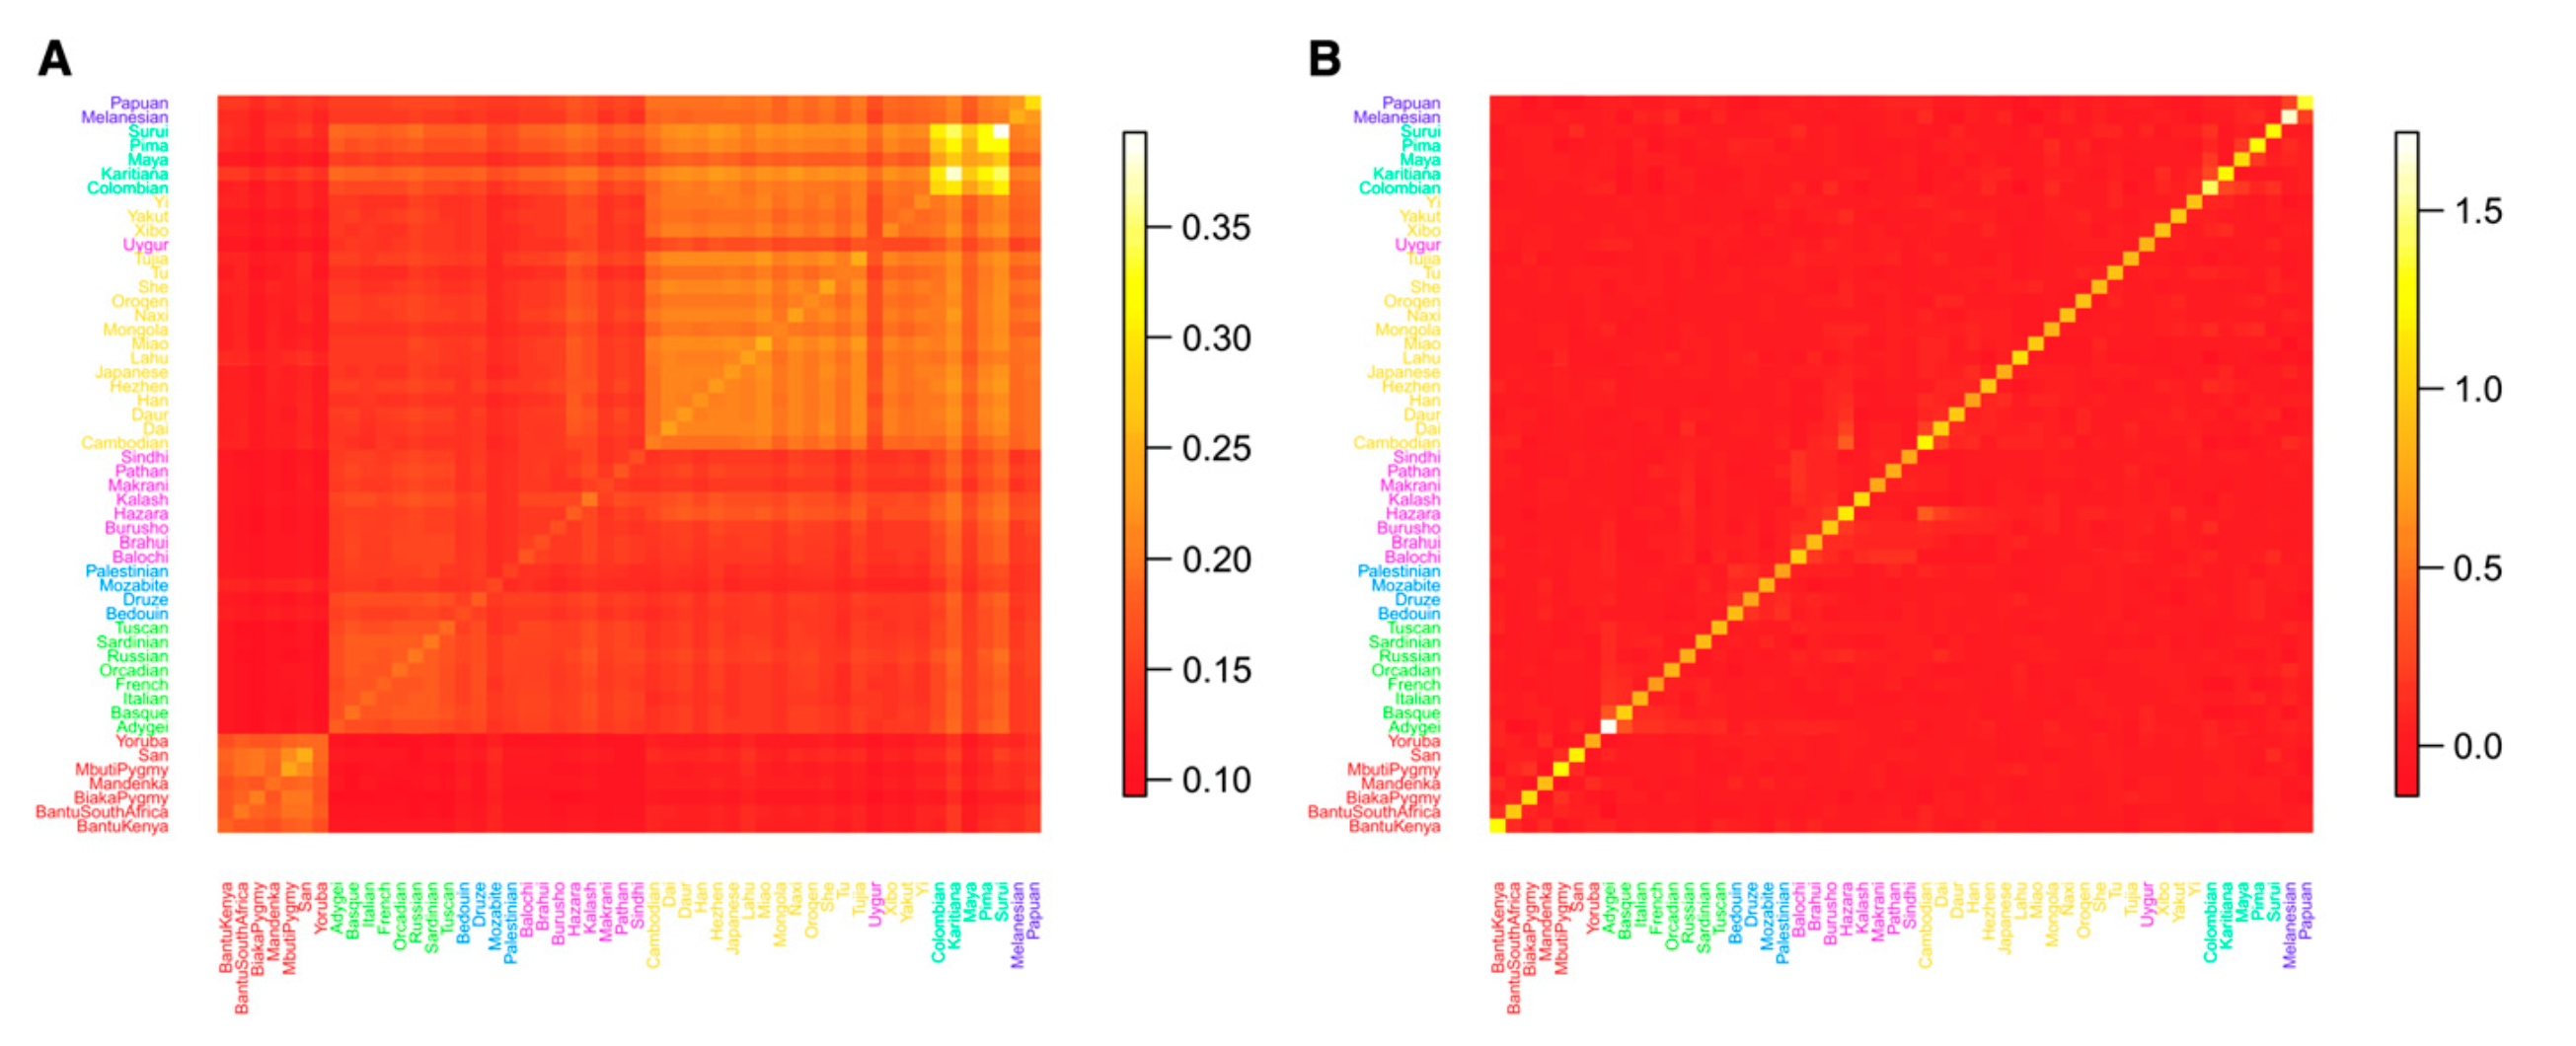
\includegraphics[width=0.8\textwidth]{xtx.png}\\
\tiny
\citet[Figure 2]{Gunther:2013ik}
\end{block}
\end{frame}

\begin{frame}
\frametitle{Bayenv: identifying correlations with ecological
variables}
\begin{block}{Input}
\centering
\begin{itemize}
\item{Allele counts}
\begin{center}
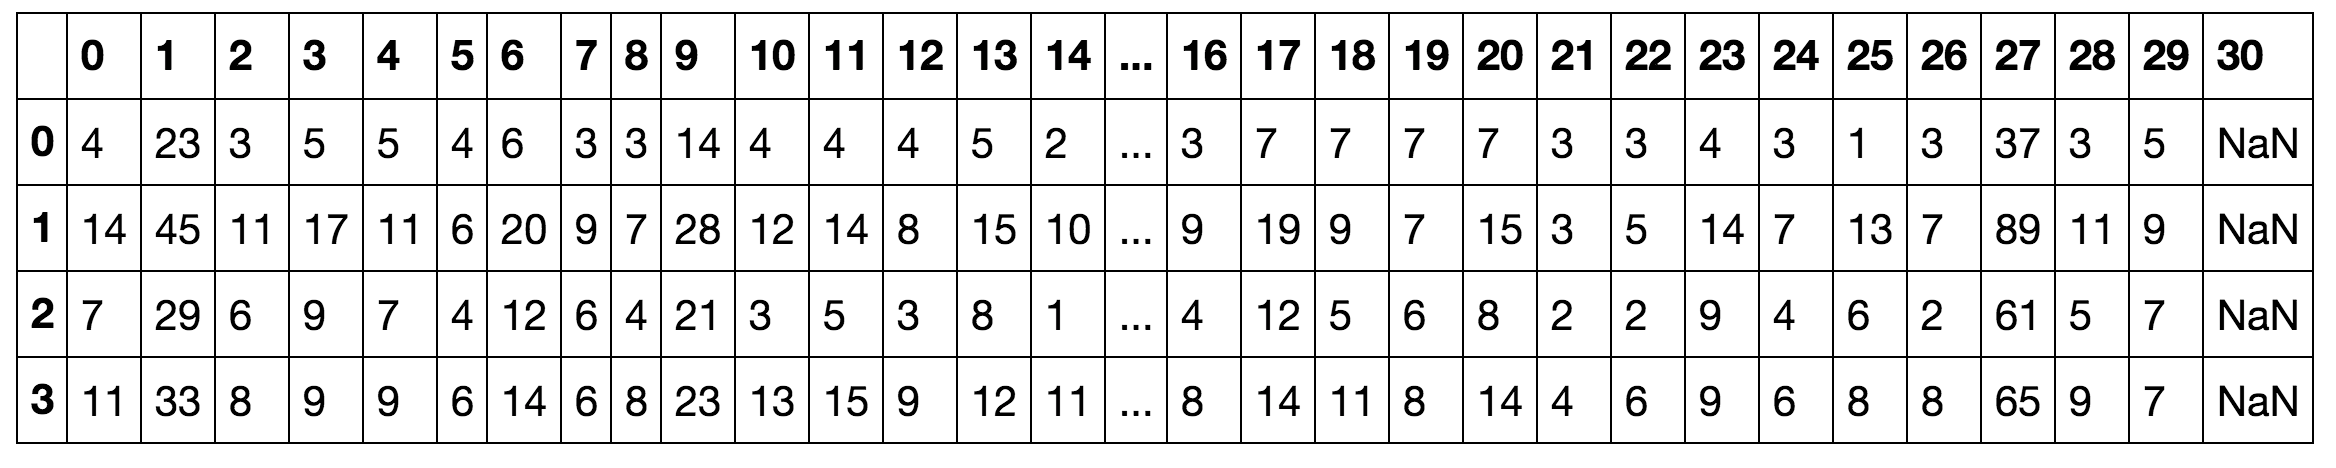
\includegraphics[width=0.8\textwidth]{bayenv_in1.png}	
\end{center}

\item{Environmental variables}
\begin{center}
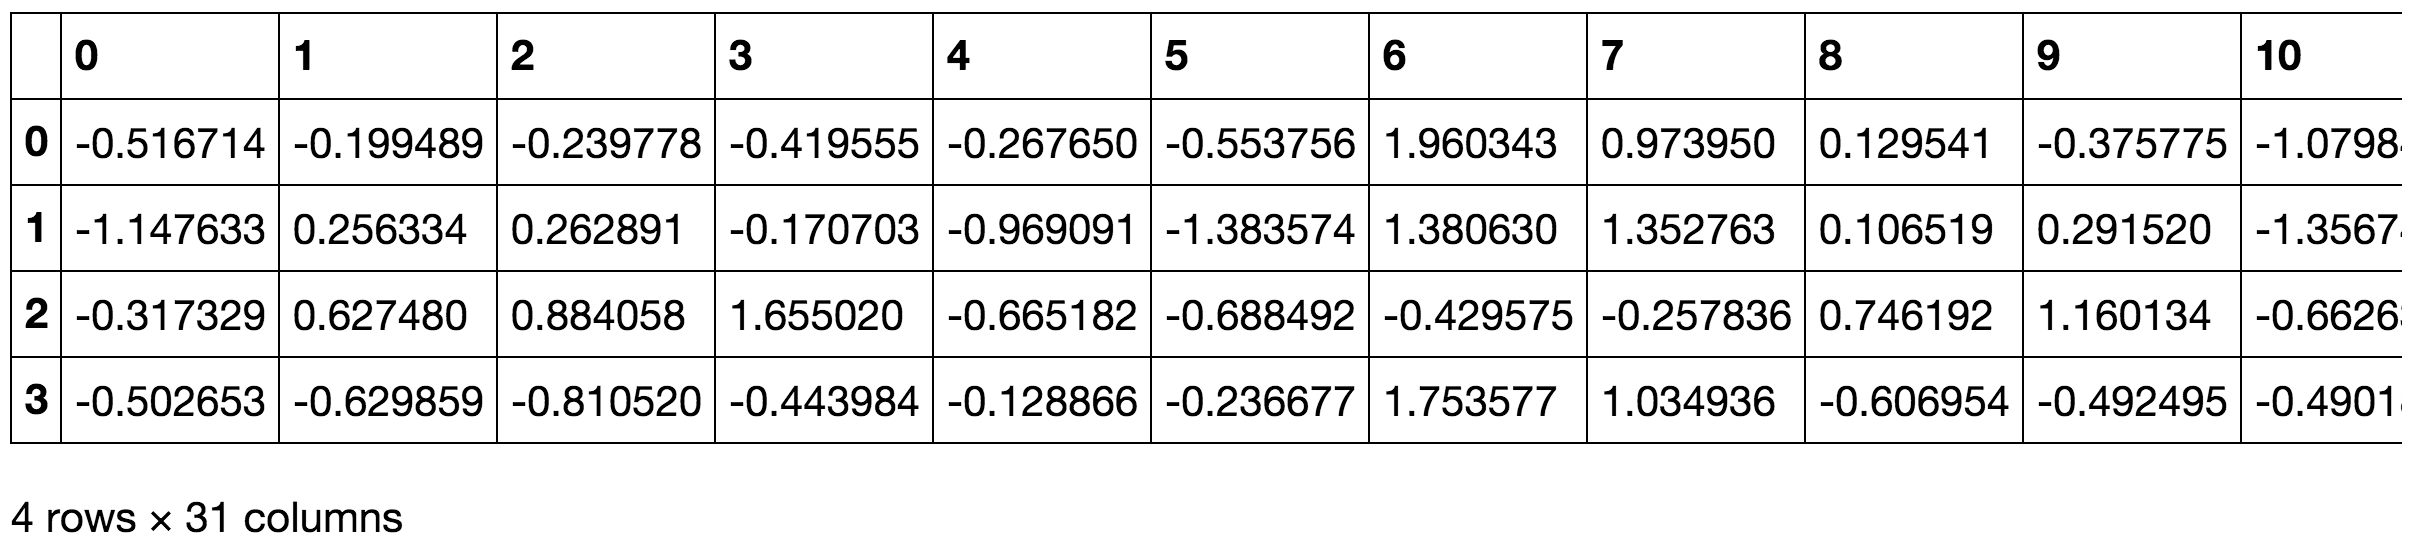
\includegraphics[width=0.8\textwidth]{bayenv_in2.png}	
\end{center}
\end{itemize}
\end{block}
\begin{block}{Question}
Do you notice a relationship between rows 0--1 and 2--3?
\end{block}

\end{frame}

\begin{frame}
\frametitle{Bayenv: identifying correlations with ecological
variables}
\begin{block}{Output}
\centering
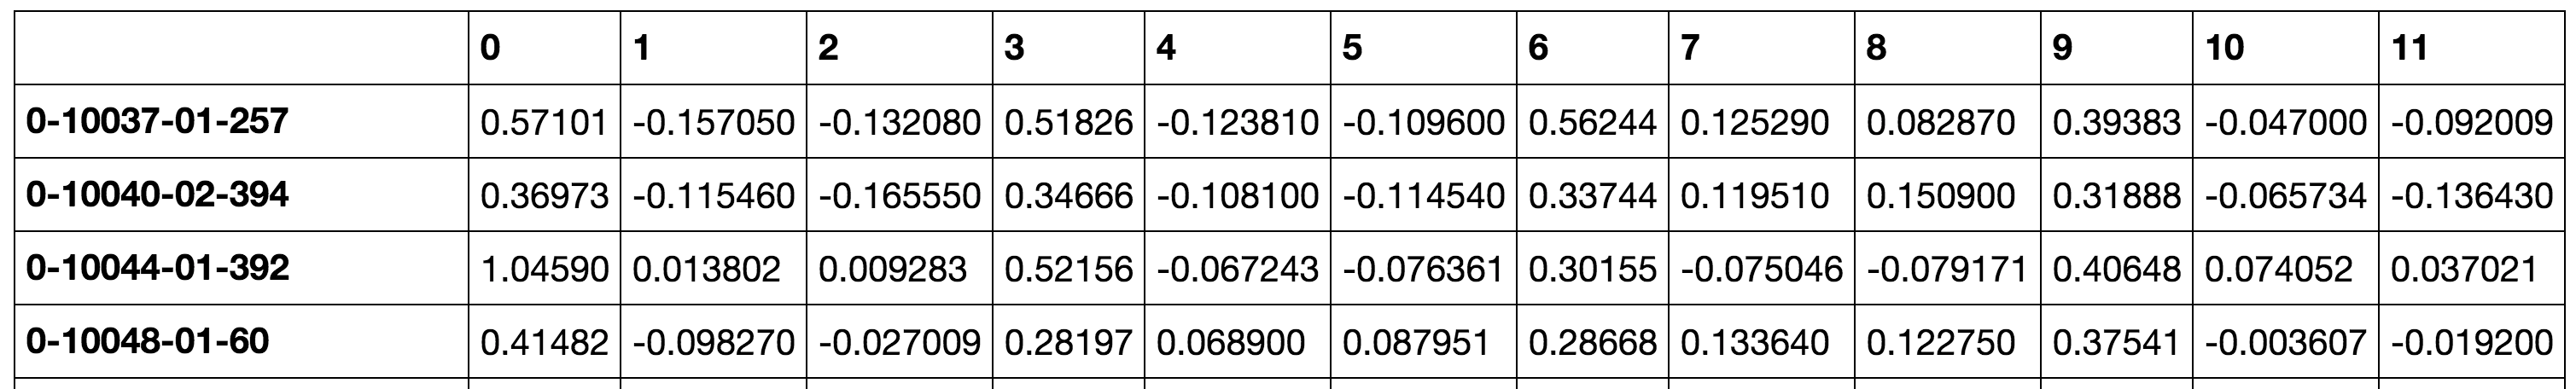
\includegraphics[width=0.8\textwidth]{bayenv_out1.png}
\end{block}
\begin{block}{Question}
Why are there 12 columns when we only input 4 environmental variables?
\end{block}

\end{frame}

\begin{frame}
\frametitle{Bayenv: identifying correlations with ecological
variables}
\begin{block}{Bayes factor outliers}
\centering
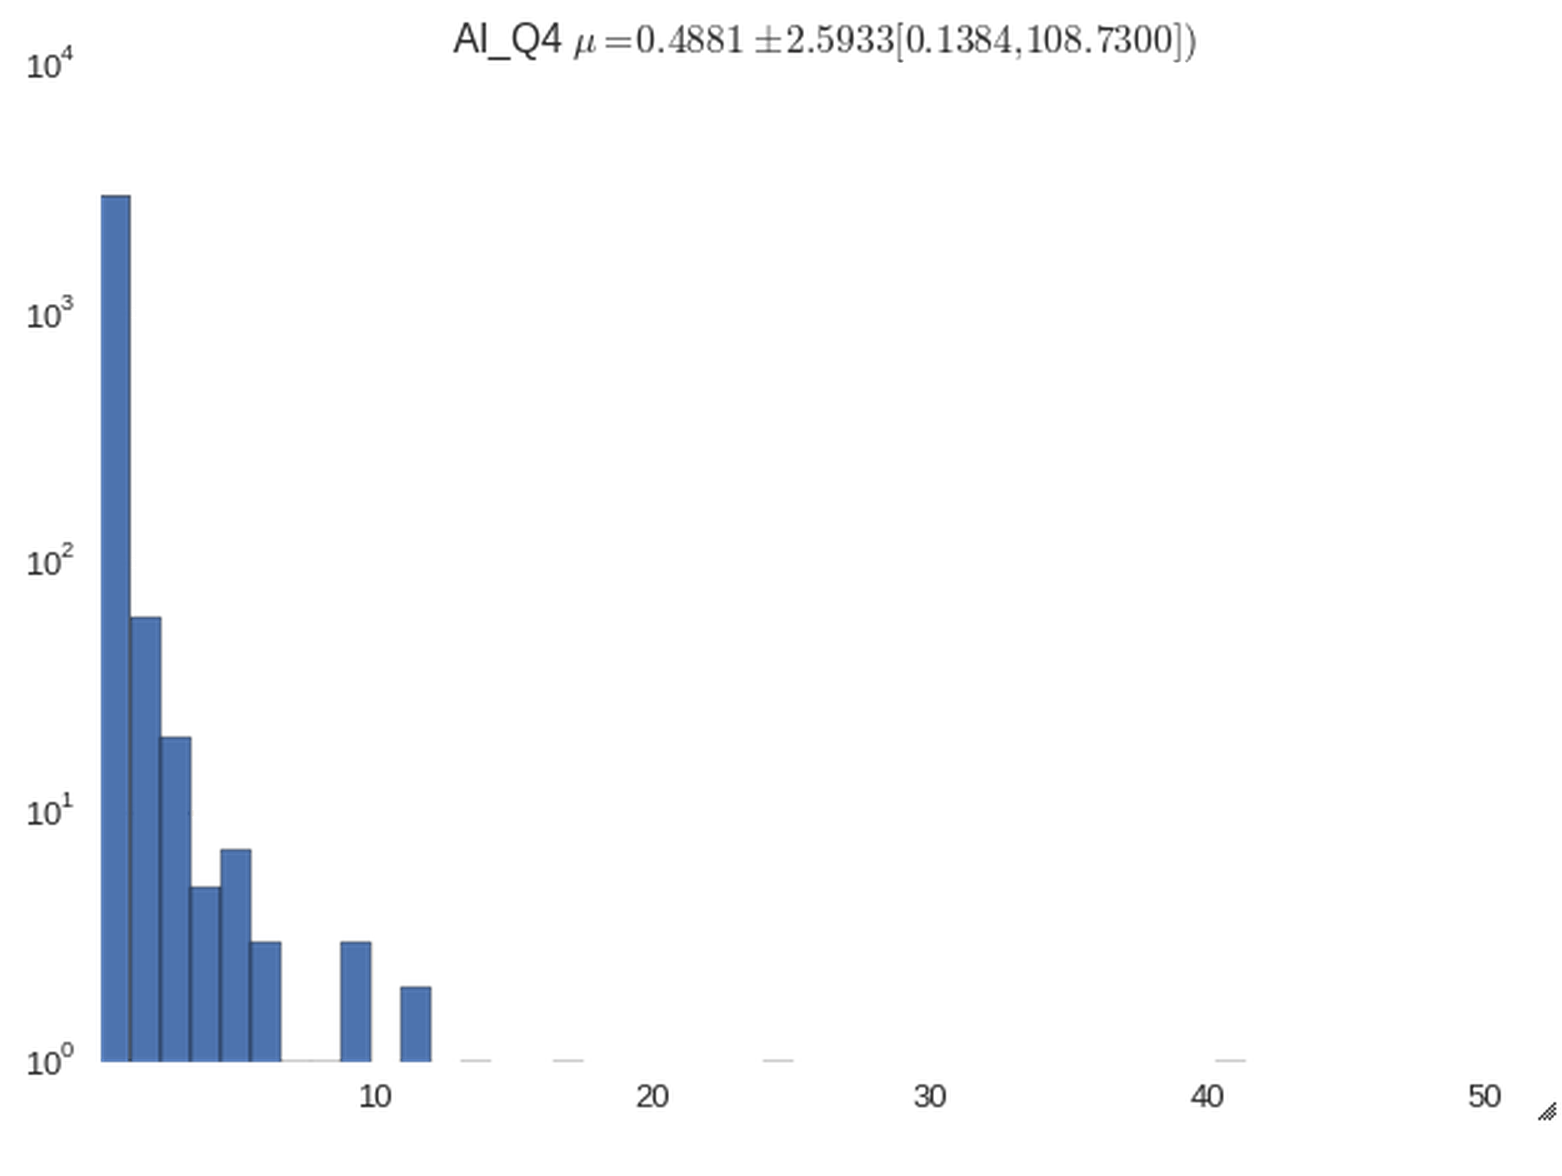
\includegraphics[height=0.6\textheight]{bayenv_outlier.png}
\end{block}
\begin{block}{Question}
How big must an outlier be? \citep{Kass:1995vb}.
\end{block}
\end{frame}



\begin{frame}
\frametitle{Signatures of polygenic adaptation}
\begin{block}{}
\centering
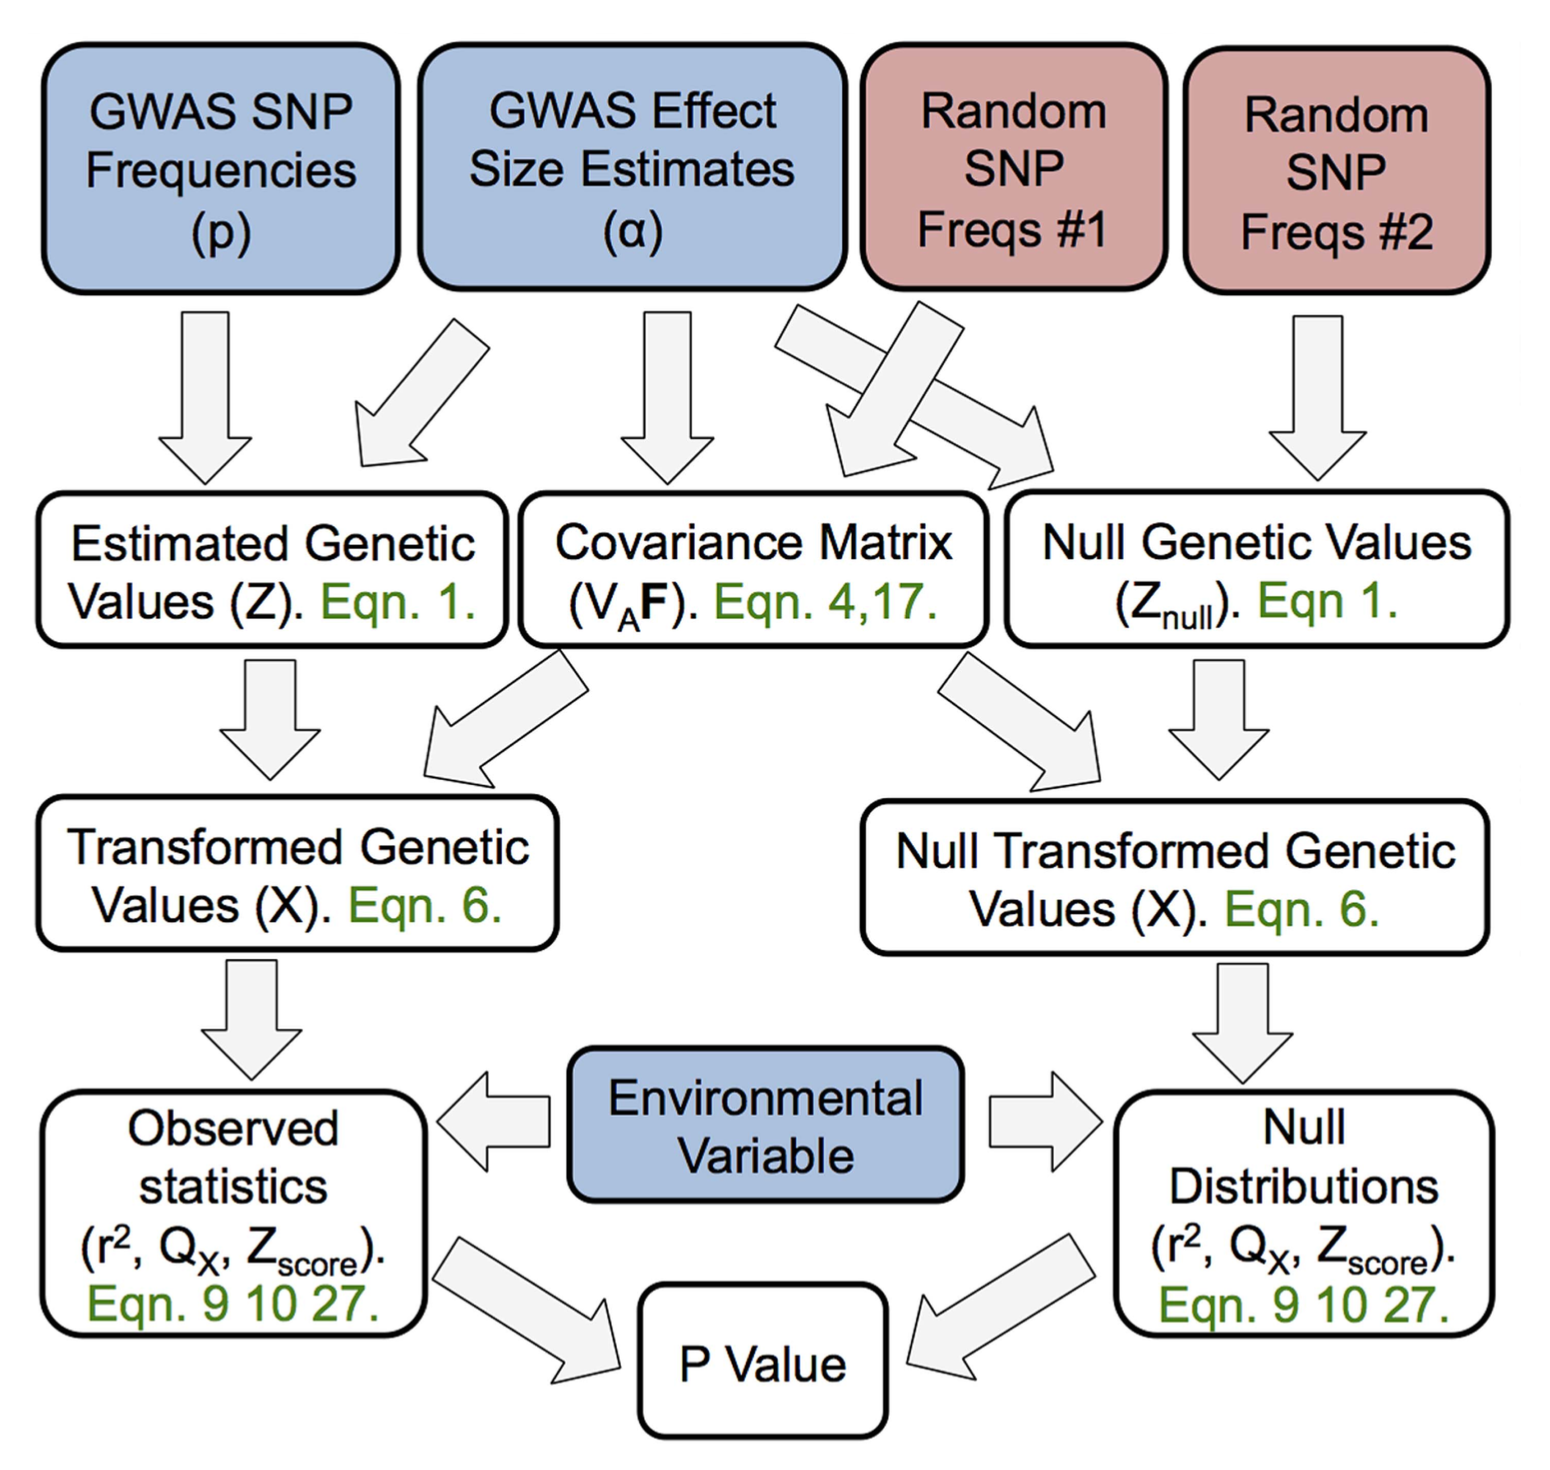
\includegraphics[height=.8\textheight]{bc1.png}
\end{block}
\tiny
\citet[Figure 1]{Berg:2014bs}
\end{frame}

\begin{frame}
\frametitle{Signatures of polygenic adaptation}
\begin{block}{}
\centering
We will not be going through all of these equations
\end{block}
\tiny
\citet[Figure 1]{Berg:2014bs}
\end{frame}

\begin{frame}
\frametitle{Signatures of polygenic adaptation}
\begin{block}{}
\centering
But...
\end{block}
\tiny
\citet[Figure 1]{Berg:2014bs}
\end{frame}

\begin{frame}
\frametitle{Signatures of polygenic adaptation}
\begin{block}{We need to calculate some values, such as $\alpha$ and $p$}
\centering
\begin{itemize}
\item{SNPassoc $\longrightarrow \alpha$}
\item{hierfstat $\longrightarrow p$}
\end{itemize}
\end{block}
\end{frame}

\begin{frame}
\frametitle{}
\begin{block}{Before we get to that, let's revisit what this method does}
\begin{itemize}
\item{The null hypothesis, unsuprisingly, is neutrality}
\item{So we can ask whether the values we observe support a role for selection,
taking into account drift and shared ancestry}
\item{Data are allele frequencies, estimates of effect size at each locus}
\item{Shared ancestry and drift are accounted for in the models}
\item{The addition of environmental variables allows testing for local
adaptation}
\end{itemize}
\end{block}
\end{frame}

\begin{frame}
\frametitle{}
\begin{block}{Qx}
Represents the variance of genetic values among populations that are not
explained by drift/demography
\begin{itemize}
\item{$\uparrow Qx$: excess of variance among populations (directional
selection/local adaptation)}
\item{$\downarrow Qx$: lack of variance among populations (stabilizing
selection)}
\end{itemize}

\end{block}
\end{frame}



\begin{frame}
\frametitle{Signatures of polygenic adaptation*}
\begin{block}{Calculating alpha, given p and q}
\centering
\begin{equation}
a = \frac{G_{AA} - G_{aa}}{2}	
\end{equation}
\begin{equation}
d = G_{Aa} - \frac{G_{AA}+G{aa}}{2}	
\end{equation}
\begin{equation}
\alpha_A = a_A + d_A(q-p)	
\end{equation}
\end{block}
\tiny
\citet{Cheverud:2015tc}
\normalsize
\begin{block}{Question}
How many genotypic classes are represented  $a$ and $d$?
\end{block}

\end{frame}



































